\chapter{Sample Memory Distribution Data-rate} \label{App:MDIST_BUSY}
This appendix shows the measured busy time of the Sample Memory Distribution module. The busy time of the module is the postive width of the signal, roughly \SIQ{80}{\nano\second}. Figure \ref{fig_App_MDIST_BUSY} shows the measured busy time, here the memory is being programemd with data at a rate of \SIQ{9.091}{\mega\hertz}.

\begin{figure}[H]
    \centering
    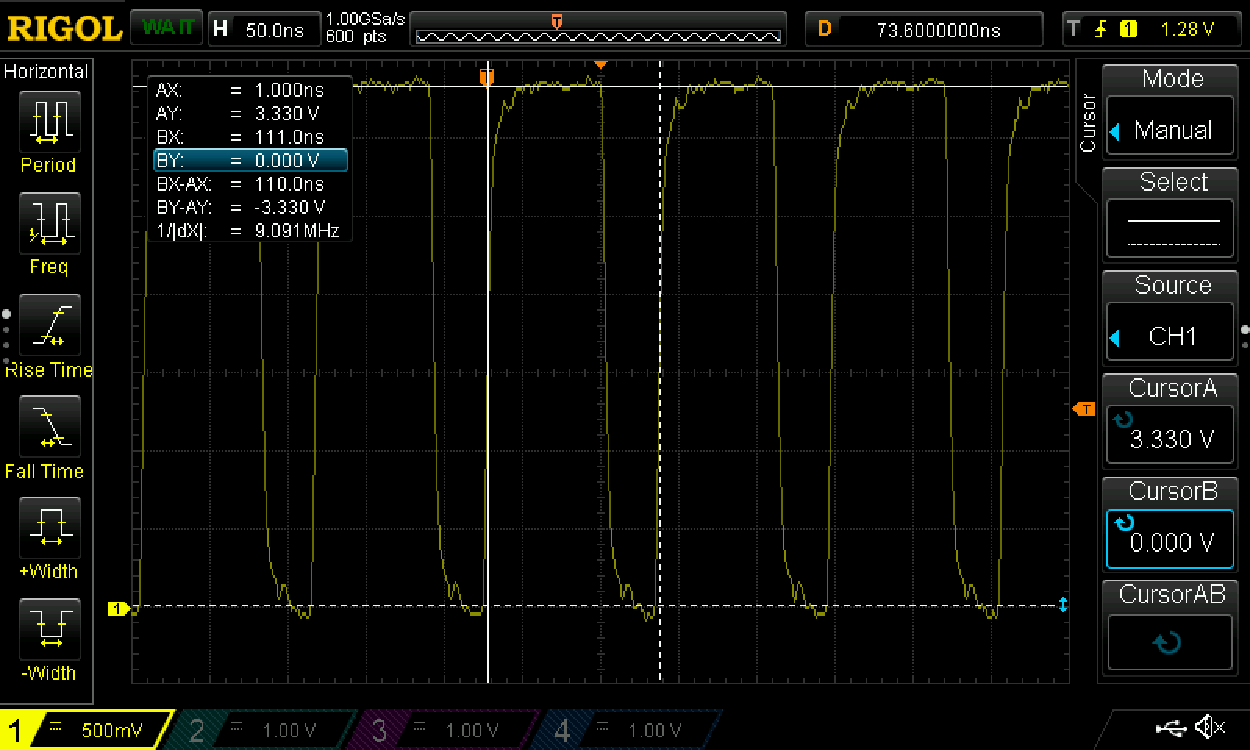
\includegraphics[clip, trim=0 0 0 0,width=1.0\textwidth]{Appendix/Figures/MDIST_BUSY.pdf}
    \caption{Busy output of the Sample Memory Distribution module, here being programmed width data at a rate of \SIQ{9.091}{\mega\hertz}, resulting in a data-rate of \SIQ{145}{\mega\bit/s}}
    \label{fig_App_MDIST_BUSY}
\end{figure}
